\documentclass[a4paper]{article}
\addtolength{\hoffset}{-2.25cm}
\addtolength{\textwidth}{4.5cm}
\addtolength{\voffset}{-3.25cm}
\addtolength{\textheight}{5cm}
\setlength{\parskip}{0pt}
\setlength{\parindent}{0in}

\usepackage[square,sort,comma,numbers]{natbib}
\usepackage{blindtext} % Package to generate dummy text
\usepackage{charter} % Use the Charter font
\usepackage[utf8]{inputenc} % Use UTF-8 encoding
\usepackage{microtype} % Slightly tweak font spacing for aesthetics
\usepackage{amsthm, amsmath, amssymb} % Mathematical typesetting
\usepackage{float} % Improved interface for floating objects
\usepackage{hyperref} % For hyperlinks in the PDF
\usepackage{graphicx, multicol} % Enhanced support for graphics
\usepackage{xcolor} % Driver-independent color extensions
\usepackage{pseudocode} % Environment for specifying algorithms in a natural way
\usepackage[mmddyy]{datetime} % Uses YEAR-MONTH-DAY format for dates

\usepackage{fancyhdr} % Headers and footers
\pagestyle{fancy} % All pages have headers and footers
\fancyhead{}\renewcommand{\headrulewidth}{0pt} % Blank out the default header
\fancyfoot[L]{} % Custom footer text
\fancyfoot[C]{} % Custom footer text
\fancyfoot[R]{\thepage} % Custom footer text
\newcommand{\note}[1]{\marginpar{\scriptsize \textcolor{red}{#1}}} % Enables comments in red on margin

\DeclareMathOperator*{\argmin}{arg\,min}

%----------------------------------------------------------------------------------------

\newcommand{\yourname}{Balthazar Neveu}
\newcommand{\youremail}{balthazarneveu@gmail.com}
\newcommand{\assignmentnumber}{3}

\begin{document}

\fancyhead[C]{}
\hrule \medskip
\begin{minipage}{0.295\textwidth} 
\raggedright
\footnotesize
\yourname \hfill\\
\youremail
\end{minipage}
\begin{minipage}{0.4\textwidth} 
\centering 
\large 
Lab session \# \assignmentnumber\\ 
\normalsize 
ALTEGRAD 2023\\ 
\end{minipage}
\begin{minipage}{0.295\textwidth} 
\raggedleft
\today\hfill\\
\end{minipage}
\medskip\hrule 
\bigskip


Assume a sequence of $L$ words (and a batch size fof $N=1$ for simplified understanding).
\section{Question 1: Role of attention and positional encoding}
\subsection*{Attention square mask}
The square mask has 2 purposes:
\begin{itemize}
\item \textbf{Causality of the prediction}: The mask serves to mask the future tokens. So the current predicted word cannot see what's coming next.
defined as a square matrix.
\item \textbf{Performances} Save some computation time during training
    \begin{itemize} 
        \item The attention scores are not computed for one word at a time. We directly let the whole sequence vector attend to the whole sequence vector, resulting
    in a $(L, L)$ attention score matrix.
        \item \textit{Note: otherwise you'd have to loop $L$ times for all the words, assume you're treating  word $l$, you have to compute an attention vector of size $l$ to the previous word.
        But tensor operations are not friendly with varying shapes. So better do a bit of extra attention computation and be able to process a whole sequence at once (actually $\frac{L*(L-1)}{2})$ useless attention scalars are computed.} 
        \item In the end, you compute a $(L,L)$ attention score and pytorch adds the mask.
        \item Adding $-\infty$ to the score will result in a weight of $0$ after the softmax operations. Basically, we do not take the future words into account when multiplying with the values.
        \item Adding $0$ to the score will leave the original weights untouched.
    \end{itemize} 


\begin{verbatim}
    Attention mask for a sequence of 5 tokens.
    10 useless computations for a sequence of 5 tokens
       [[0., -inf, -inf, -inf, -inf],
        [0.,   0., -inf, -inf, -inf],
        [0.,   0.,   0., -inf, -inf],
        [0.,   0.,   0.,   0., -inf],
        [0.,   0.,   0.,   0.,   0.]]
\end{verbatim}
\end{itemize} 


\subsection*{Positional encoding}
The role of positional encoding is to provide the order of the words in the sentence to the attention mechanism.
\begin{itemize}
\item Observation 1: \textit{Order in a sequence matters: "Le chat chasse la souris" has a totally different meaning that "La souris chasse le chat".}
\item Observation 2: \textit{Unlike recurrent neural networks (RNNs) like the GRU-based architecture we used in lab 1 for translation, the Transformer \cite{vaswani2017} architecture \cite{vaswani2017}
doesn't process source sentences in a step-by-step manner. Instead, it processes all tokens in the sequence simultaneously.
This parallel processing capability gives Transformer \cite{vaswani2017}s their efficiency but also means that they lack an inherent sense of position or order in a sequence.}
\item To solve the issue mentioned above, positional encoding vector is added to the embeddings of tokens before they're fed into the Transformer \cite{vaswani2017}.
The positional encoding is a set of values that's designed to give the model information about the position of each token within the sequence.
The goal is to ensure that the resulting combined embeddings (token embedding + positional encoding) will be unique for each position, even if the token is the same.
\item This also lets the Transformer \cite{vaswani2017} architecture (in its internal computations) behave differently depending on the "distance" between words.
\end{itemize} 

\section{Question 2: Classification head}
\subsection*{Language modeling}
During pre-training, the Transformer \cite{vaswani2017} model transforms each token into a representative feature vector supposed to model the next word.

The classification head used for this purpose maps that vector into a logit/probability of getting the next word.
This allows to train on a corpus of un-annotated
sentences. If you want to generate new text or complete a sequence, you can use this classifier. \newline
But \textbf{if you want to do any other downstream task} (e.g sentiment classification or spam classification)
\textbf{the original classifier becomes useless.}

\subsection*{Downstream task(like classification)}
Instead, you can replace the original classification head dedicated to language modeling by a new classification head for a specific downstream task. 

To fine-tune, we can basilly freeze the Transformer \cite{vaswani2017} pretrained weigths and leverage the fact that the representation outputs of the Transformer \cite{vaswani2017}
will model the tokens in a very sensitive feature space. A powerful feature space which models many inherent things in the sentence.
Therefore, with a few annotated data samples for your downstream classification task (e.g Google maps comments on restaurants annotated with their star ratings, spam/not spam examples), you can simply retrain a new classifier head.
\textit{Freezing the Transformer \cite{vaswani2017} weights is not mandatory, you could also fine tune the Transformer \cite{vaswani2017} layers... but it seems a bit risky in my opinion if there's not much data
to perform the downstream task training.} 

\pagebreak
\section{Question 3: Trainable parameters}

\subsection*{Notations}


\begin{itemize}
    \item $V$ is the vocabulary size
    \item $D$ is the hidden feature dimension which is also equal to the embedding dimension: \textit{hdim} $=$ \textit{embeddingDim} for simplifications.
    \item $M$ is the number of attention layers.
    \item $A$ is the number of attention heads (denoted $h$ in \cite{vaswani2017}).
    \item $C$ is the number of classes.
\end{itemize}

\subsection*{Parameters computation}


\begin{equation}
\begin{aligned}
\text{Total number of parameters} =\\
\underbrace{V.D}_{\text{embedding look up table}} \\
+ M*\big[
\underbrace{\overbrace{3}^{\text{Key,Query,Value}} *
(A*\big(\overbrace{D*\frac{D}{A}}^{\text{weights}} + \overbrace{\frac{D}{A}}^{\text{bias}})\big)}_{\text{Linear embeddings projection}}
+ \underbrace{(\overbrace{D^2}^{\text{weights}} + \overbrace{D}^{\text{bias}})}_{\text{Weighted values linear projection after concatenation}} \\
+ \underbrace{2* (\overbrace{D^2}^{\text{weights}} + \overbrace{D}^{\text{bias}})}_{\text{2 chained feedforward netwoks}}
+ \underbrace{2*(\overbrace{D}^{\text{slope}}+\overbrace{D}^{\text{offset}})}_{\text{2 layer normalizations}}
    \big] \\
+ \underbrace{\overbrace{D*C}^{\text{weights}} + \overbrace{C}^{\text{bias}}}_{\text{classifier head}} \\
= V.D + M*\big[ 6D^2+ 10D\big] + C(D+1)
\end{aligned}
\end{equation}


We're able to cross check:
\begin{itemize}
    \item the number of parameters returned by the pytorch \textit{numel} function
    \item the analytical computation using \textit{sympy} for symbolic computation in python.
\end{itemize}
Let's check a simple example with a single layer ($M=1$).
\begin{tiny}
\begin{verbatim}

+-------------------------------------------------------------+------------+---------------------+------------------+
|                           Modules                           | Parameters | Analytic validation | Analytic formula |
+-------------------------------------------------------------+------------+---------------------+------------------+
|                     base.encoder.weight                     |  10000200  |       10000200      |       D*V        |
|  base.transformer_encoder.layers.0.self_attn.in_proj_weight |   120000   |        120000       |       3*D²       |
|   base.transformer_encoder.layers.0.self_attn.in_proj_bias  |    600     |         600         |       3*D        |
| base.transformer_encoder.layers.0.self_attn.out_proj.weight |   40000    |        40000        |        D²        |
|  base.transformer_encoder.layers.0.self_attn.out_proj.bias  |    200     |         200         |        D         |
|       base.transformer_encoder.layers.0.linear1.weight      |   40000    |        40000        |        D²        |
|        base.transformer_encoder.layers.0.linear1.bias       |    200     |         200         |        D         |
|       base.transformer_encoder.layers.0.linear2.weight      |   40000    |        40000        |        D²        |
|        base.transformer_encoder.layers.0.linear2.bias       |    200     |         200         |        D         |
|        base.transformer_encoder.layers.0.norm1.weight       |    200     |         200         |        D         |
|         base.transformer_encoder.layers.0.norm1.bias        |    200     |         200         |        D         |
|        base.transformer_encoder.layers.0.norm2.weight       |    200     |         200         |        D         |
|         base.transformer_encoder.layers.0.norm2.bias        |    200     |         200         |        D         |
|                  classifier.decoder.weight                  |  10000200  |       10000200      |       C*D        |
|                   classifier.decoder.bias                   |   50001    |        50001        |        C         |
+-------------------------------------------------------------+------------+---------------------+------------------+
\end{verbatim}
\end{tiny}

\break


\subsection*{Language modeling vs classification}


Let's take an example
\begin{itemize}
    \item $V= 50001$
    \item $D= 200$ hidden feature dimension or embeddings dimension
    \item $M= 4$ is the number of attention layers.
    \item $A= 2$ is the number of attention heads (but it does not affect parameters compution)
\end{itemize}

We have 2 configurations:
\begin{itemize}
    \item Language modeling: $C \text{ classes}=V \text{ vocabulary size}$ 
    \item Sentiment classification: $C \text{ classes}= 2$ (good/bad) 
    \item Here we'll assume that for the classification fine tuning, the transformer backbone (embeddings+ transformer layers) 
    is totally frozen and that we only train the classifier's weights. This is a very lightweight fine tuning.
\end{itemize}
\begin{table}[h]
    \begin{tabular}{|l|l|l|}
    \hline
    \multicolumn{1}{|c|}{Number of trainable parameter}              & \multicolumn{1}{c|}{Language modeling task $C=V$} & \multicolumn{1}{c|}{Classification task $C=2$}                                                       \\ \hline
    \begin{tabular}[c]{@{}l@{}}Word embeddings\end{tabular} & Trainable $V.D$                                   & \multicolumn{1}{c|}{\begin{tabular}[c]{@{}c@{}}$0$ trainable parameters\\ = Frozen  \end{tabular}} \\ \hline
    $M$ Transformer layers with $A$ heads                                           & Trainable $M*\big[ 6D^2+ 10D\big]$                           & \begin{tabular}[c]{@{}l@{}}$0$ trainable parameters\\ = Frozen \end{tabular}                      \\ \hline
    Classifier head                                                  & Trainable  $V(D+1)$                                 & Trainable       $2(D+1)$                                                                                \\ \hline   
    Total (analytics) & $V.D + M*\big[ 6D^2+ 10D\big] + C(D+1)$ & $2(D+1)$ \\ \hline
    Total parameter & 21M parameters (21018401) & $402$ parameters  \\ \hline
\end{tabular}
\end{table}

\subsection*{Remark on the number of attention heads}
Please note that due to the tricky implementation of torch,
$A$ does not appear in the final computation (chunk Key $K$, Query $Q$ and Value $V$ into $D$ chunks of  size $\frac{D}{A}$ ).
This allows keeping the same computation budget with various attention heads.
This explicitly appears in the \href{https://github.com/pytorch/pytorch/blob/main/torch/nn/modules/activation.py#L990}{pytorch source code}
of MultiheadAttention
\begin{verbatim}
    self.head_dim = embed_dim // num_heads
\end{verbatim}

\section*{Task 3}
\begin{verbatim}
    <sos> Comment montrer que je suis autonome .
    Comment montrer que je suis autonome . <eos>
\end{verbatim}

Training logs. Seems like everything is going fine.
On a Nvidia T500, there is a memory limitation, we have to limit the sentence length to avoid out of memory issues.


\begin{itemize}
    \item $batch_{size} = 16$
    \item $max_{len} = 64$
\end{itemize}

\begin{verbatim}
    | epoch   1 |   500/ 3125 steps | loss 7.29929 | ppl 1479.254
    | epoch   1 |  1000/ 3125 steps | loss 6.47710 | ppl  650.081
    | epoch   1 |  1500/ 3125 steps | loss 6.19202 | ppl  488.834
    | epoch   1 |  2000/ 3125 steps | loss 6.05407 | ppl  425.842
    | epoch   1 |  2500/ 3125 steps | loss 5.93240 | ppl  377.057
    | epoch   1 |  3000/ 3125 steps | loss 5.82976 | ppl  340.279
    | epoch   2 |   500/ 3125 steps | loss 5.50992 | ppl  247.131
    | epoch   2 |  1000/ 3125 steps | loss 5.46325 | ppl  235.864
    | epoch   2 |  1500/ 3125 steps | loss 5.42948 | ppl  228.032
    | epoch   2 |  2000/ 3125 steps | loss 5.40475 | ppl  222.461
    | epoch   2 |  2500/ 3125 steps | loss 5.37446 | ppl  215.824
    | epoch   2 |  3000/ 3125 steps | loss 5.35723 | ppl  212.136
\end{verbatim}



Here are the prediction results compared to the provided pretrained model.

\begin{verbatim}
Epoch 2:
--------
Bonjour les plus tard, il a été mis à la fin de la région de la Commission,
mais aussi de la loi de la région de la Commission

Pretrained model:
-----------------
Bonjour les gens qui ont été très accueillants et sympathiques.
\end{verbatim}


\section{Question 4: Results interpretation}
We train on 1600 sentences for the downstream task of sentiment analyzis, which is a classification task (good/bad review).
Some nitty gritty details on the implementation:
\begin{itemize}
    \item "Taking the last word feature vector" does not mean take the last element of the tensor output of the model. For each batch element, 
you need to retrieve the last word before padding.
    \item I removed the mask to let each word access the whole sentence... there may be a tiny discrepancy with regard to the original Language modeling task
as the pretrained transformer may not be used to see some words "in the future". I tried both solutions by the way, picked what felt right...
it didn't change the training curves much by the way.
\end{itemize}

\begin{figure}[ht]
    \centering
    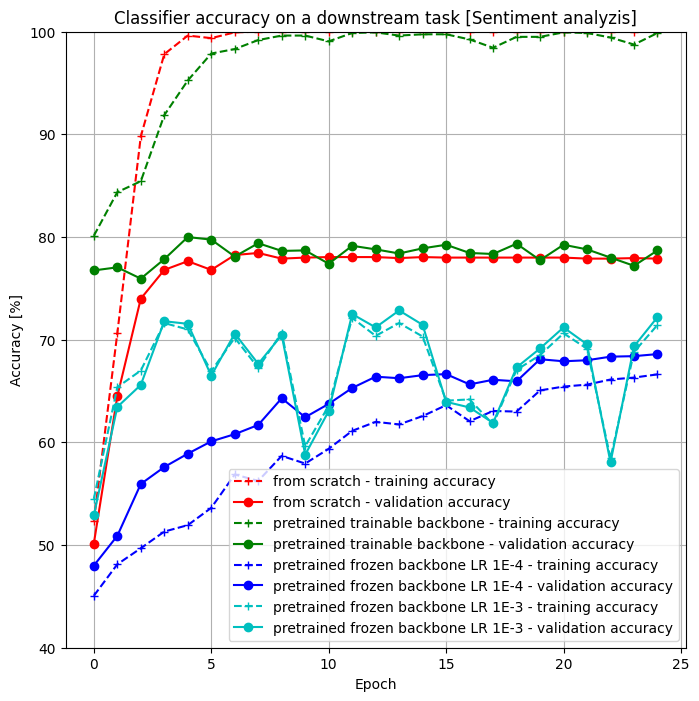
\includegraphics[width=.6\textwidth]{figures/accuracy_curves_bugfixed.png}
    \caption{Training and validation accuracies for different setups (start from scratch, pretrained model, 
    frozen pretrained model to only train the lightweight classifier)}
    \label{fig:training_curve}
\end{figure}


From \ref{fig:training_curve}, we can see that starting the classification training from a pretrained transformer model on the language modeling task
works gets much better accuracy in a single epoch than training a model initalized randomly. $76\% >> 65\%$ after 2 epoch. This is quite incredible and
This can be explained by the fact that the feature vectors learnt on the language modeling task are very versatile and definitely contain a lot
of semantic information.
We see that if we'd taken the best fine tuned pretrained model at epoch=5, we get $80\%$ accuracy when pretraining from scratch goes to $78\%$ (slower but
still an remarkable performance).
These training curves also show that in a few epochs, we're able to memorize the whole training dataset (training accuracy goes to $100\%$, loss goes to zero)
as shown by the dashed red and green curves. With 20M parameters, it's not a surprise. These classifiers may lack a bit of the skill to generalize.
They may memorize some easy "words" or patterns to recognize whether or not a review is positive or not.
I also tried to freeze the transformer weights (blue and cyan curves), this training goes faster as there are only a few parameters to train
in the classifier head (see Question 3 with the assumption I made for the fine-tuning stage)... but the accuracy is not as great.  This still avoids
the memorization of the training set.

Let's take a look at some results using the fine tuned model based on the pretrained Transformer.
\begin{figure}[ht]
    \centering
    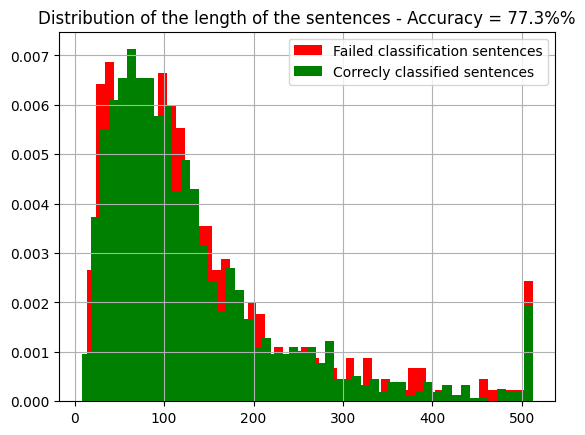
\includegraphics[width=.6\textwidth]{figures/distribution_of_sentences_length.png}
    \caption{Distribution of the length of the sentences when classifier fails or succeed... there's no obvious gap here.}
    \label{fig:length_distribution}
\end{figure}
Finally in \ref{fig:length_distribution}, we show that there's no easy analyzis to make like "the model is unable to classify long sentences"...
as basically the distribution of sentences length looks the same whether or not they're classified correctly or wrongly.

Some samples of fail below to see some concrete examples where the model failed. These are not so easy as you can see.
\begin{verbatim}
GROUNDTRUTH=NEGATIVE -> PREDICTION= POSITIVE
je ne recommande absoluement pas ce torchon , véritable offense 
à la mémoire de Michael Jackson . Il repose enfin en paix ...
\end{verbatim}
"repose enfin en paix" may still be difficult to classify as it's not a "bad" sentiment but a respectful sentence.
"torchon" and "offense" are strong words where a model shall not fail and consider it as negative feelings.

\begin{verbatim}
GROUNDTRUTH=POSITIVE -> PREDICTION= NEGATIVE #
ce livres et une vrai drogue ! la derniere fois je n' arrivais meme pas a m' arreter 
! A LIRE ABSOLUMENT !!!! !!!! !!!! !!!
\end{verbatim}
"Drogue" may have biased the result toward the negative prediction.



\section{Question 5: Language modeling limitations}
\begin{itemize}
\item The proposed approach to language modeling is next word prediction which implies causality. It is also known as autoregressive language modeling.
Example: "Salut les copains, comment ???"
\item BERT \cite{devlin2019bert} introduces a different training objective which is masked language modeling. 
Example: "Salut les copains, ??? allez vous?"
\end{itemize}

In the causal LM objective, each token can only attend to previous tokens in the sequence, it's unidirectional. 
This is because the model is designed to predict the next token in a sequence. 
While this setup is great for generative tasks, it doesn't always capture the context from both sides (before and after) 
of a word or phrase, which can be beneficial for understanding its meaning in certain situations.

A comment might begin negatively but end positively or vice versa. Being able to see and consider the entire sentence at once can help in better grasping its overall sentiment.
Example: "L'ensemble du livre est médiocre. Mais les dix premières pages m'ont vendu tellement de rêve que je l'ai lu jusqu'au bout."
The classifier based on the autoregressive language model may simply forget the begining of the sentence and classify the review as a "good review".
The BERT model will actually have to focus on both the negative and positive sentences to actually understand the "Mais" word.

\subsection*{Note}
\textit{
For the specific downstream task considered in this notebook, sentiment classification, 
it didn't seem straigthforward at first that we'd need the bidirectional advantage
of BERT to simply grasp whether or not the recommendation was good or not. It doesn't seem like a very complete.
BERT\cite{devlin2019bert} shines on much more complex reasoning benchmarks examples mentioned in the GLUE \cite{wang2019glue} benchmark like
the Winograd canonical example:} \\
Who does the pronoun \textbf{They} refer to in the 2 following sentences?.

\begin{itemize}
\item \textbf{The city councilmen} refused the demonstrators a permit because \textbf{they} feared violence.
\item The city councilmen refused \textbf{the demonstrators} a permit because \textbf{they} advocated violence.
\end{itemize}

Answering this question definitely requires the context before and after the word \textbf{they} and seems much more
complex than feeling what's negative or positive in a review.
%------------------------------------------------

\bibliographystyle{plain}
\bibliography{references} % citation records are in the references.bib document

\end{document}